% -*- program: xelatex -*-
\documentclass[UTF8]{ctexart}
\usepackage{minted}
\usepackage{hyperref}
\usepackage{url}

\title{卷积码编码译码器的设计}
\author{常增禄 \\ 无36 \\ 2013011188 \and
        李思涵 \\ 无36 \\ 2013011187 \and
        沈睿哲 \\ 无36 \\ 2013011185}
\date{2017年1月1日}
\begin{document}
\maketitle

\section{实验原理}

卷积码是信道编码的一种,其工作方式是将输入信号和编码器的冲激响应进行卷积操作,故得名卷积码。
与分组编码不同,卷积码具有记忆性。
维特比译码则是利用了动态规划的思想,可用于卷积码的译码。

在本次实验中,我们决定在仿真平台上搭建卷积码编码译码器。
为了提高实验的难度,我们在实现编码器和译码器的同时实现调制和解调,从而实现一个完整的端到端的通信系统。

\section{小组分工}

本次实验的小组分工如下:

\begin{description}
    \item[常增禄] 负责调制/解调部分的代码实现;
    \item[李思涵] 负责卷积码编码部分的代码实现,各模块的整合;
    \item[沈睿哲] 负责维特比译码部分的代码实现。
\end{description}
\section{系统设计}

\subsection{卷积码编码}

我们考虑实现一个图~\ref{fig:213} 所示的 (2, 1, 3) 卷积码。
其中,我们使用移位寄存器来保存状态,使用异或运算来产生输出信号,从而实现卷积码的编码操作。

\subsection{调制/解调}

我们选择使用 FSK 调制,将基带信号调制到两个高频载波上,通过控制载波的频率来传输信息。
在接受端,我们则选择通过计数器的方式来识别不同频率的载波,从而达到解调的目的。

\subsection{维特比译码}

我们考虑的是以下(2,1,3)卷积码,如图~\ref{fig:213} 所示。

\begin{figure}[htbp]
    \centering
    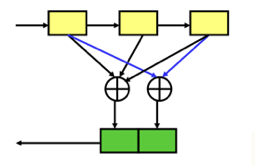
\includegraphics[width=0.5\textwidth]{figs/213}
    \caption{(2,1,3)卷积码}
    \label{fig:213}
\end{figure}

由此我们可以画出状态图,如图~\ref{fig:statuses} 所示(状态和编码均是按上图的从左至右写)。

\begin{figure}[htbp]
    \centering
    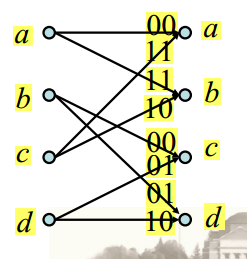
\includegraphics[width=0.5\textwidth]{figs/statuses}
    \caption{(2,1,3)卷积码状态图}
    \label{fig:statuses}
\end{figure}

从0状态开始,可以做出我们的网格图,如图~\ref{fig:status_network} 所示。

\begin{figure}[htbp]
    \centering
    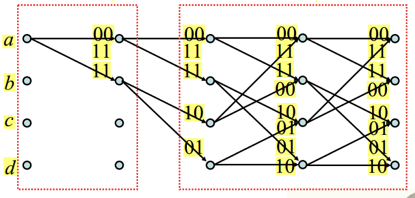
\includegraphics[width=0.5\textwidth]{figs/status_network}
    \caption{(2,1,3)卷积码网格图}
    \label{fig:status_network}
\end{figure}

由于寄存器数目有限,我们不可能对无线长度的码一直保存其代价和路径。
所以我们考虑7个为开窗(这样代价正好可以用三比特描述)。
又由于每七个码的最后步骤需要比较四个节点的代价并选取最终路径,计算过程很难直接在单个周期内完成,需要额外延时一个周期,所以我们采用人工归零状态的策略。
即对于每组的七位待编码,将每五个待编码后面加两个零作为补偿一起构成七位待编码:XXXXX00。
这样就可以不用额外用一个周期进行计算。


\section{代码实现}

\subsection{文件清单}

本次实验以及报告的源代码可以在 \url{https://github.com/ThomasLee969/convolutional-coding} 找到。
这里列出实验所需代码如下。

\begin{minted}[linenos]
conv_encoder.v
conv_encoder_tb.v
demodulator.v
main.v
main_tb.v
modulator.v
modulator_tb.v
viterbi.v
viterbi_tb.v
watchmaker.v
\end{minted}


\subsection{卷积码编码}

\inputminted[linenos]{verilog}{../src/conv_encoder.v}

可以看到,我们利用一个长度为 3 的移位寄存器保存状态,并利用状态位之间的异或操作产生输出。
需要注意的是,由于这里编码器的输出比特率是输入比特率的两倍,我们在这里使用了两个时钟信号,一个作为输入信号时钟,一个作为输出信号时钟。

\subsection{调制/解调}

\subsubsection{调制}

\inputminted[linenos]{verilog}{../src/modulator.v}

调制采用FSK调制,将基带传输信号“0”,“1”调制到两个高频率的载波上.
此处为方便生成,选择了clk信号的8分频信号和16分频信号作为两个载波频率。

设置1个3位计数器,clk上升沿计数。
计数到4时,8分频信号反向;计数到8时,8分频和16分频信号反向,同时计数器清零。

对于串行2进制数据流,接收“1”输出8分频信号,接收“0”输出16分频信号。

\subsubsection{信道}

仿真时采用理想无失真信道,不考虑误码的影响,直接将调制的输出连接到解调的输入上。

后面为测试解码性能添加误码时,为了方便也不在信道处添加误码,而选择在编码后添加。

\subsubsection{解调}

\inputminted[linenos]{verilog}{../src/demodulator.v}

对接收信号的上升沿个数计数。
由于接收信号为clk的8分频和16分频的混合信号,在16个clk信号的周期内,8分频有2个上升沿,而16分频只有1个上升沿,由此可以解调,得到原信号。

\subsection{维特比译码}

\subsubsection{接口,寄存器声明部分}
\inputminted[linenos, firstline=7, lastline=26]{verilog}{../src/viterbi.v}

\subsubsection{译码路径逻辑部分}
分别计算下一个状态为a,b,c,d的代价和译码路径,大量重复的以下代码:
\inputminted[linenos, firstline=173, lastline=312]{verilog}{../src/viterbi.v}

\subsubsection{输出部分}
\inputminted[linenos, firstline=390, lastline=418]{verilog}{../src/viterbi.v}

\section{仿真结果}

\subsection{调制/解调}

\begin{figure}[htbp]
    \centering
    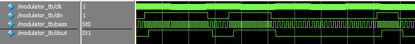
\includegraphics[width=0.95\textwidth]{figs/modulation-sim}
    \caption{调制/解调仿真结果}
    \label{fig:modulation-sim}
\end{figure}

调制/解调模块的仿真结果如图~\ref{fig:modulation-sim} 所示。

\subsection{整体仿真结果}

\begin{figure}[htbp]
    \centering
    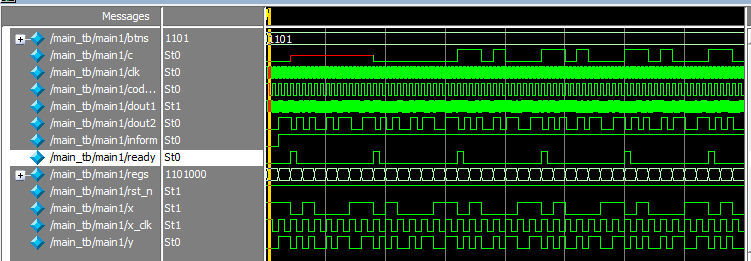
\includegraphics[width=0.95\textwidth]{figs/sim}
    \caption{整体仿真结果}
    \label{fig:sim}
\end{figure}

整体仿真结果如图~\ref{fig:sim} 所示。
我们不断循环输入1101000作为待编码,
可以看到x是输入待编码的码:1101000
y是编码后的码:11010100101100
c是译码结果,在ready的上升沿为首位开始读取:1101000
c=x,译码正确。


\section{实验结果}

我们将编译好的程序上传至了实验平台上。
为了验证我们实现的正确性,我们先用 1011 作为输入,并将输出端接至示波器。
示波器上的波形输出如图~\ref{fig:correct} 所示。
可以看到,我们确实得到了 1011 的输出。
这说明我们的编码,调制,解调和译码的过程都是正确的。

\begin{figure}[htbp]
    \centering
    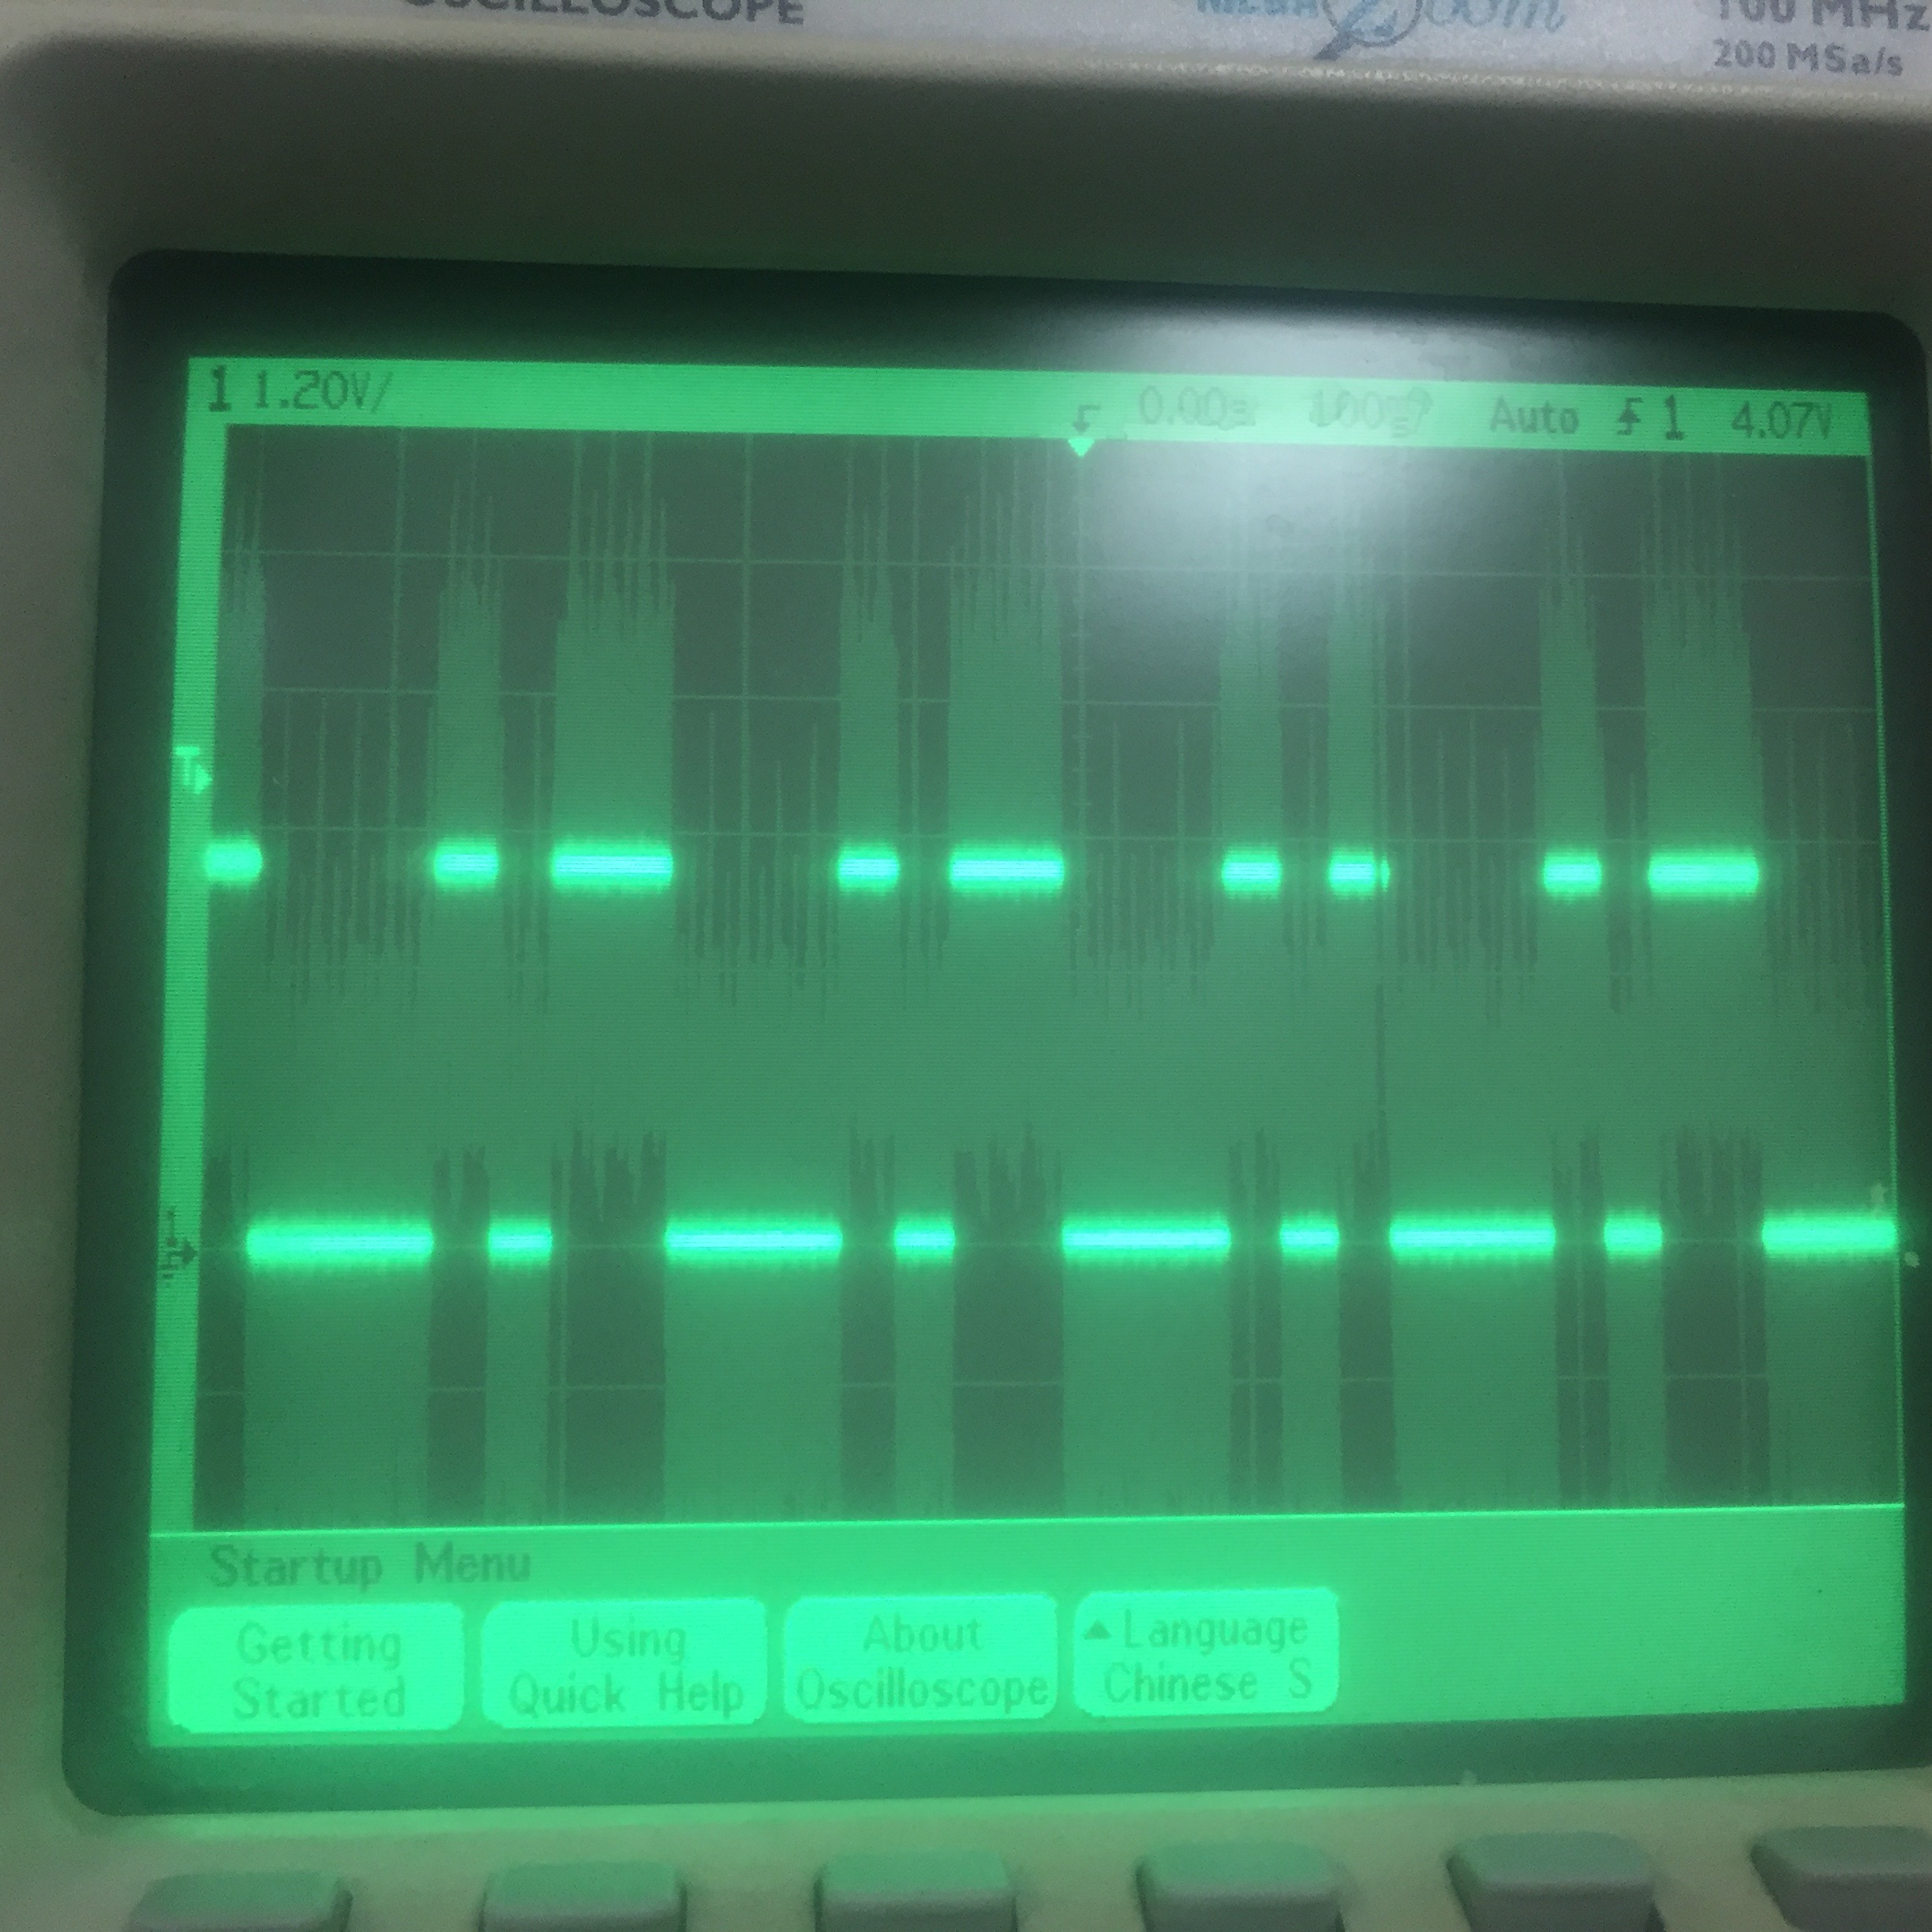
\includegraphics[width=0.7\textwidth]{figs/correct}
    \caption{实验结果}
    \label{fig:correct}
\end{figure}

同时,我们还测试了过量误码对系统的影响。我们修改了调制模块,让其每 3 比特误码一次。
实验的结果如图~\ref{fig:wrong} 所示。
可以看到,加入过量误码后系统不仅不能正常工作,其输出甚至不能保证原来的周期。
这是因为在加入了误码后,维特比译码不能在每一个周期之后恢复到零状态,故其整体周期会有所延长。

\begin{figure}[htbp]
    \centering
    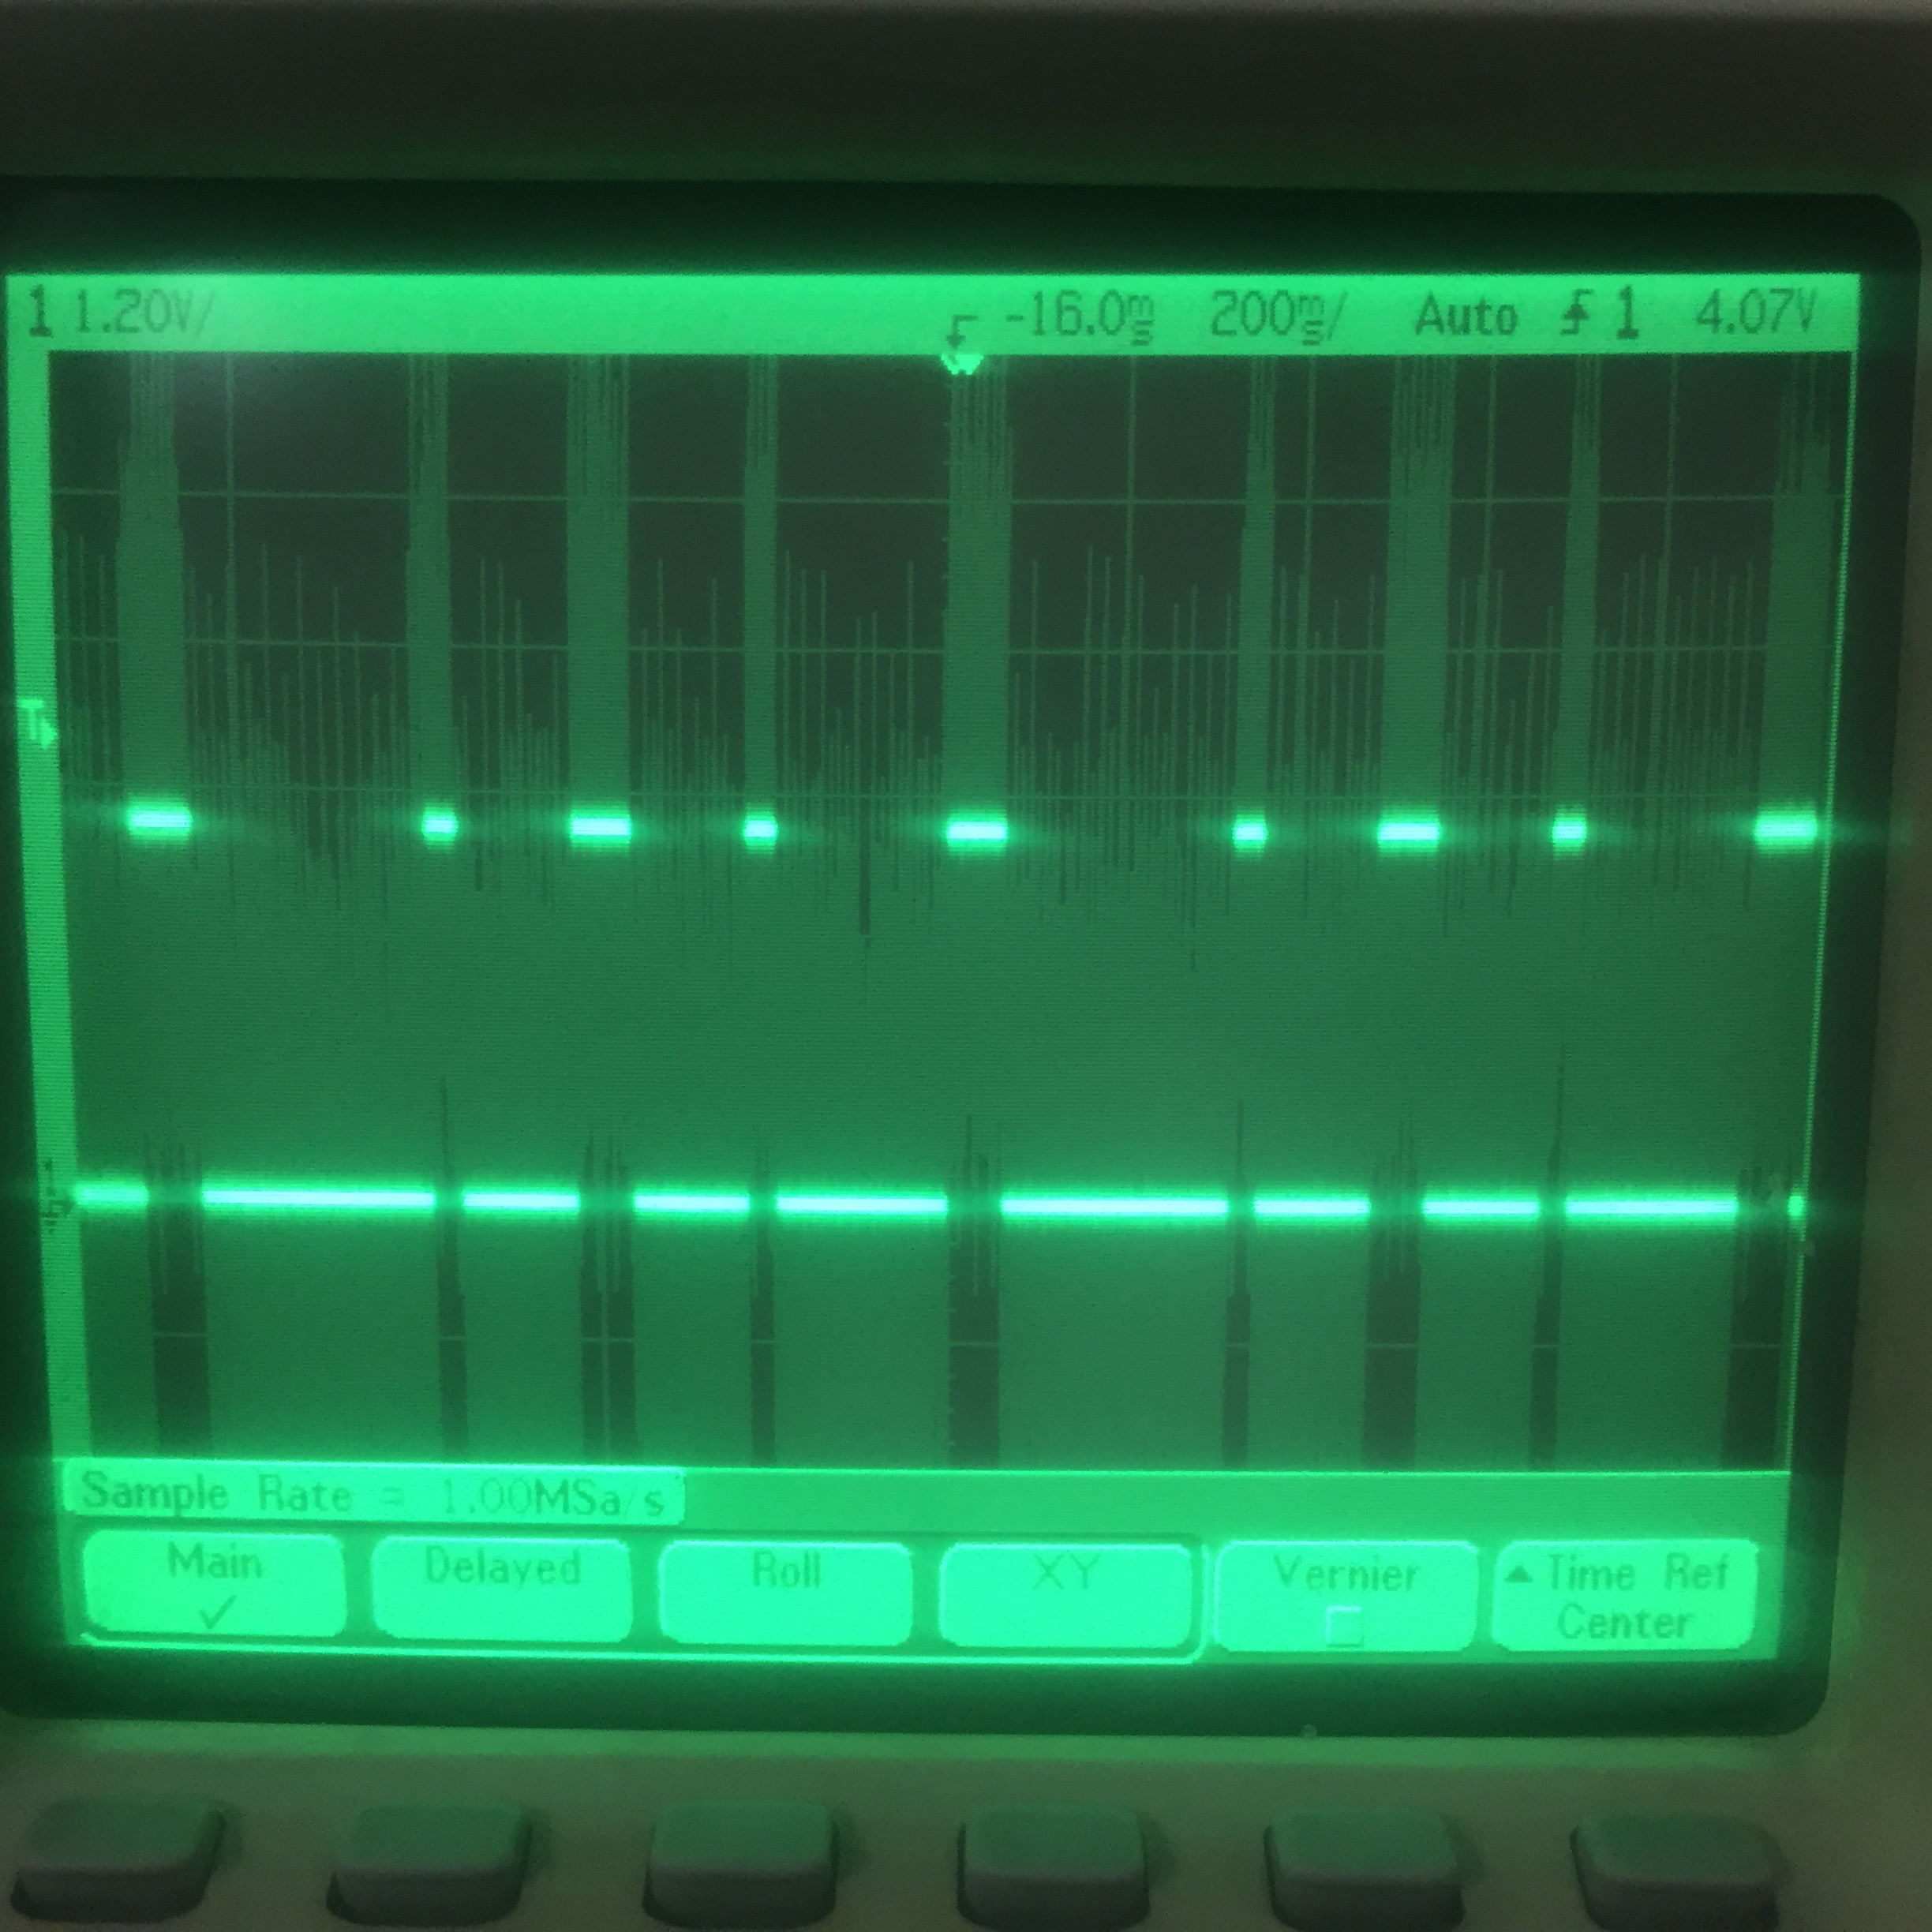
\includegraphics[width=0.7\textwidth]{figs/wrong}
    \caption{加入过量误码后的实验结果}
    \label{fig:wrong}
\end{figure}


\section{实验总结}

在本次实验中,我们从零开始,在仿真平台上搭建了一套能够正常工作的通信系统。
在实验的过程中,我们发现最难的一点是代码在硬件上的调试。
有很多次,我们发现我们的代码在仿真时没有问题,但是一上传到仿真平台上就不能正常工作。
之后的检查发现,这种问题多半是因为在写代码时依赖了一些时序,初值等方面的假设,而这些假设在硬件平台上不一定成立。
然而,一个通信系统最终是要落实在硬件上的。所以,硬件上的调试和仿真时的调试同样重要。

\end{document}
